\documentclass[12pt]{article}
\usepackage{amsmath, amssymb}
\usepackage{tikz}

\begin{document}

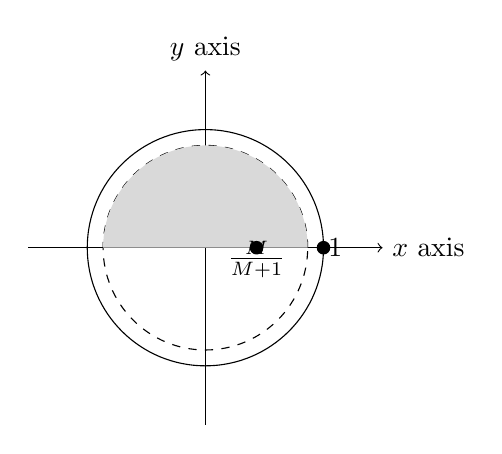
\begin{tikzpicture}[scale=1.5]
    % Draw the coordinate axes
    \draw[->] (-1.5,0) -- (1.5,0) node[right] {$x$ axis};
    \draw[->] (0,-1.5) -- (0,1.5) node[above] {$y$ axis};
    
    % Draw the outer circle
    \draw (0,0) circle (1);
    
    % Draw the inner circle with dashed line
    \draw[dashed] (0,0) circle (0.866);
    
    % Fill the shaded region
    \fill[gray!30] (0.866,0) arc (0:180:0.866) -- cycle;
    
    % Mark the point (M/(M+1), 0)
    \filldraw[black] (0.433,0) circle (1.5pt);
    \node at (0.433, -0.1) {$\frac{M}{M+1}$};
    
    % Label the point (1,0)
    \filldraw[black] (1,0) circle (1.5pt);
    \node at (1.1, 0) {1};
\end{tikzpicture}

A Stolz type region $\{ z \in \mathbb{D} : |1 - z|^2 < M(1 - |z|^2) \}$.

\end{document}